\documentclass{beamer}
%
% Choose how your presentation looks.
%
% For more themes, color themes and font themes, see:
% http://deic.uab.es/~iblanes/beamer_gallery/index_by_theme.html
%
\mode<presentation>
{
  \usetheme{Madrid}      % or try Darmstadt, Madrid, Warsaw, ...
  \usecolortheme{beaver} % or try albatross, beaver, crane, ...
  \usefonttheme{default}  % or try serif, structurebold, ...
  \setbeamertemplate{navigation symbols}{}
  \setbeamertemplate{caption}[numbered]
} 

\usepackage[english]{babel}
\usepackage[utf8x]{inputenc}
\usepackage{graphicx}
\usepackage{listings}

\lstset{
	breaklines=true,
	escapeinside={(*@}{@*)}
}

\graphicspath{{img/}}

\title[State Space Search Algorithms]{State Space Search Algorithms}
\author{Vedran Pintarić}
\date{8.11.2018.}

\begin{document}

\begin{frame}
  \titlepage
\end{frame}

\section{Problem definition}

\begin{frame}{Problem definition}

	\begin{itemize}
		\item a set of states (state space)
		\item initial state
		\item transitions between states
		\item goal state test
	\end{itemize}

\end{frame}

\begin{frame}[fragile]{Problem definition}

	\begin{lstlisting}[language=Python]
class Problem:
  # Should return a State object
  def getInitialState(self):
    pass

  # Should check if given
  # state is goal state
  def isGoalState(self, state):
    pass

  # Should return a list
  # of triplets (state, action, cost)
  def getSuccessors(self, state):
    pass
	\end{lstlisting}

\end{frame}

\subsection{8-Puzzle}

\begin{frame}
	\begin{figure}
	\centering
		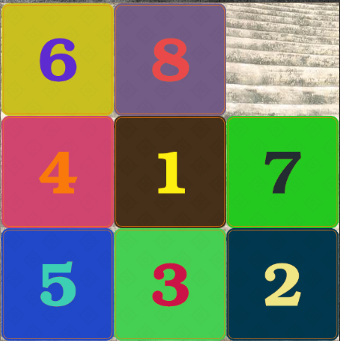
\includegraphics[width=0.5\linewidth]{puzzle8.png}
		\caption{8-Puzzle initial state}
	\end{figure}
\end{frame}

\begin{frame}
	\begin{figure}
	\centering
		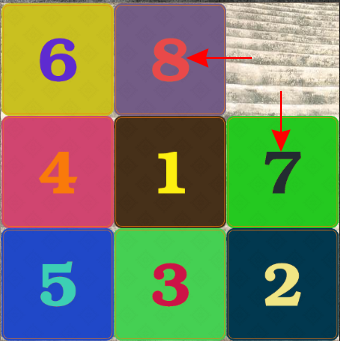
\includegraphics[width=0.5\linewidth]{puzzle8_arrows.png}
		\caption{8-Puzzle possible actions}
	\end{figure}
\end{frame}

\begin{frame}
	\begin{figure}
	\centering
		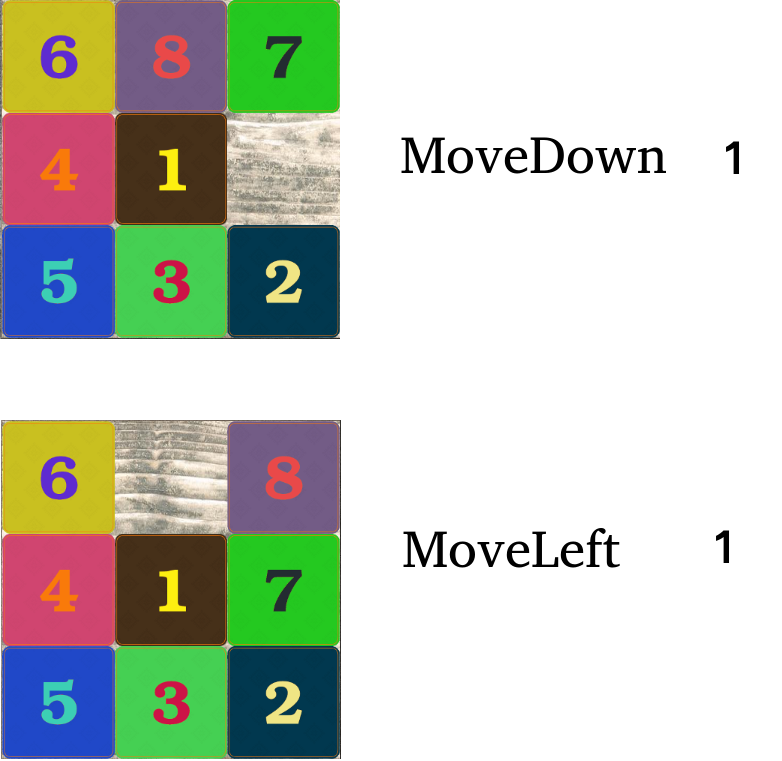
\includegraphics[width=0.5\linewidth]{puzzle8_successors.png}
		\caption{8-Puzzle list of successor triplets}
	\end{figure}
\end{frame}

\begin{frame}
	\begin{figure}
	\centering
		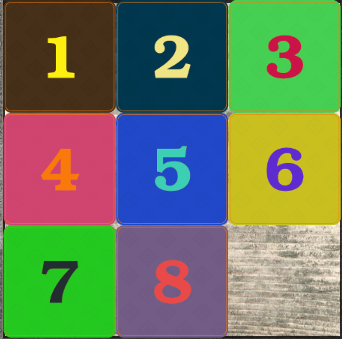
\includegraphics[width=0.5\linewidth]{puzzle8_goal.png}
		\caption{8-Puzzle goal state}
	\end{figure}
\end{frame}

\subsection{Pathfinding}

\begin{frame}
	\begin{figure}
	\centering
		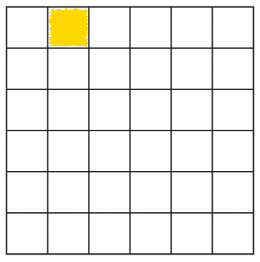
\includegraphics[width=0.5\linewidth]{pathfinding.png}
		\caption{Pathfinding initial state}
	\end{figure}
\end{frame}

\begin{frame}
	\begin{figure}
	\centering
		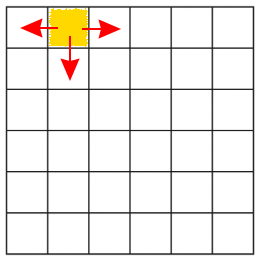
\includegraphics[width=0.5\linewidth]{pathfinding_arrows.png}
		\caption{Pathfinding possible actions}
	\end{figure}
\end{frame}

\begin{frame}
	\begin{figure}
	\centering
		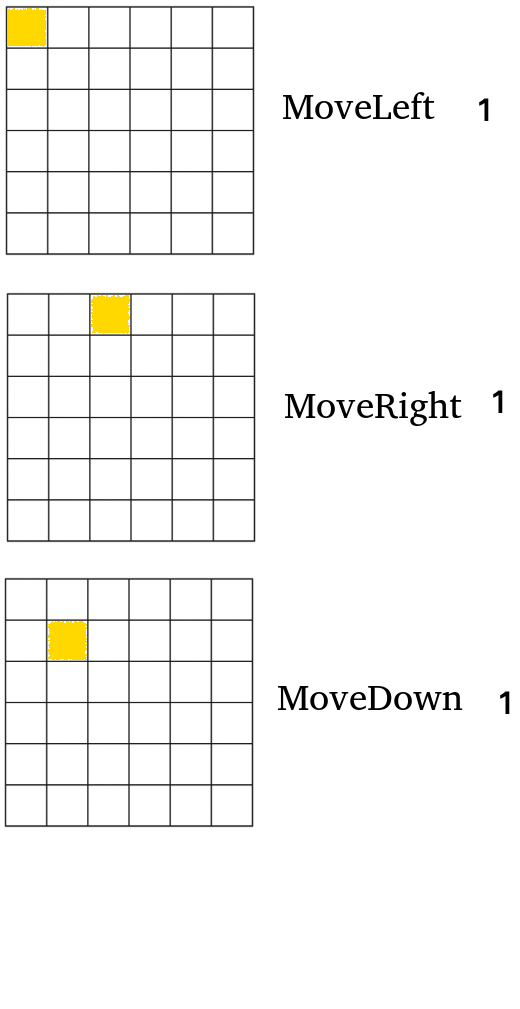
\includegraphics[width=0.3\linewidth]{pathfinding_successors.png}
		\caption{Pathfinding list of successor triplets}
	\end{figure}
\end{frame}

\begin{frame}{State space graph}
	\pause
	\begin{figure}
	\centering
		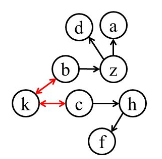
\includegraphics[width=0.6\linewidth]{state_space_graph.png}
		\caption{State space graph}
	\end{figure}
\end{frame}

\section{Search algorithm}

\subsection{Search tree}

\begin{frame}{Search tree}

	\begin{figure}
	\centering
		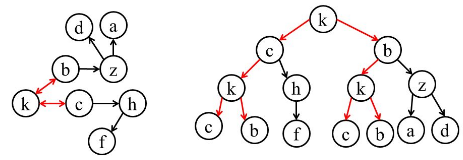
\includegraphics[width=\linewidth]{state_space_vs_search_tree.png}
		\caption{State space vs search tree}
	\end{figure}

\end{frame}

\begin{frame}{Nodes}

	\begin{itemize}
		\item Open nodes - known but unexplored
		\item Closed nodes - explored i.e. checked against goal state and their successors were queried
	\end{itemize}

\end{frame}

\subsection{General algorithm pseudocode}

\begin{frame}[fragile]{General algorithm pseudocode}
	\begin{lstlisting}
closedNodes = {}
openNodes = {}

openNodes.insert(getInitialState())
while openNodes not empty 
  node = openNodes.get()
  if isGoalState(node)
    return node
		
  if node in closedNodes
    continue
	
  for childNode in getSuccessors(node)
    if childNode not in closedNodes
      openNodes.insert(childNode)
  closedNodes.insert(node)
	\end{lstlisting}
\end{frame}

\section{Blind algorithms}

\begin{frame}{Working example}

	\begin{figure}
	\centering
		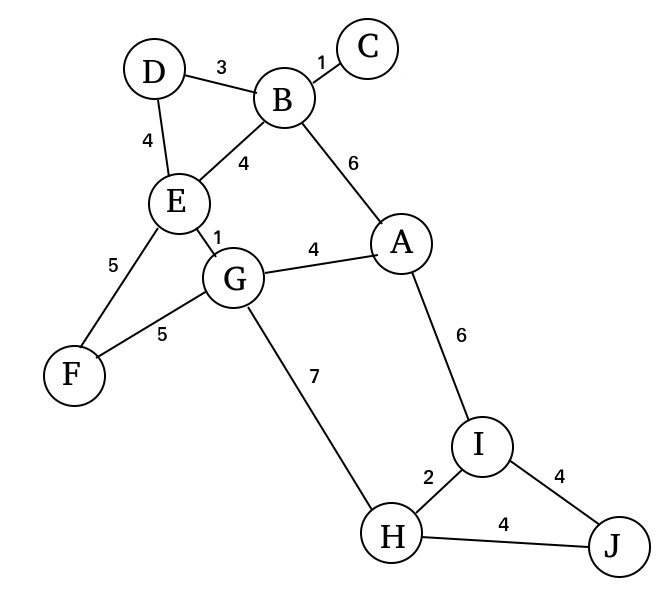
\includegraphics[width=0.75\linewidth]{example.jpg}
	\end{figure}

\end{frame}

\begin{frame}{Blind algorithms}

	\begin{columns}[T]
	
		\begin{column}{.48\textwidth}
			\begin{figure}
			\centering
				
\includegraphics[width=\linewidth]{spongebob_blind.jpg}
			\end{figure}
		\end{column}
		
		\begin{column}{.48\textwidth}
		
			\begin{itemize}
				\item no additional information about the problem
				\item needs to figure everything out on it's own
			\end{itemize}
		
		\end{column}
	
	\end{columns}

\end{frame}

\subsection{Breadth first search (BFS)}

\begin{frame}[fragile]{Breadth First Search (BFS)}
	\begin{lstlisting}
closedNodes = {}

# First In First Out
openNode = Queue()

openNodes.insert(getInitialState())
while openNodes not empty 
  node = openNodes.get()
  if isGoalState(node)
    return node
  if node in closedNodes
    continue				
  for childNode in getSuccessors(node)
    if childNode not in closedNodes
      openNodes.insert(childNode)
  closedNodes.insert(node)
	\end{lstlisting}
\end{frame}

\begin{frame}{Breadth First Search (BFS)}
	\begin{columns}[T]
		\begin{column}{.48\textwidth}
			\begin{figure}
			\centering
				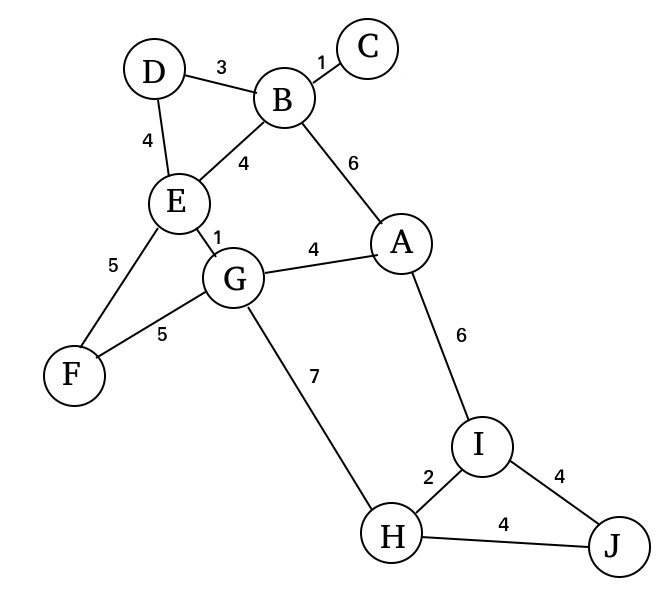
\includegraphics[width=1.3\linewidth]{example.jpg}
			\end{figure}
		\end{column}
		
		\begin{column}{.48\textwidth}
				\begin{itemize}
					\item Find a path from B to I
					\newline
					\only<1>{
						\item OPEN: {[ B ]}
						\newline
						\item CLOSED: \{\}
					}
					\only<2>{
						\item OPEN: {[ \textcolor{blue}{C, D, E, A} ]}
						\newline
						\item CLOSED: \{ \textcolor{red}{B} \}					
					}
					\only<3>{
						\item OPEN: {[ D, E, A ]}
						\newline
						\item CLOSED: \{ B, \textcolor{red}{C} \}
					}
					\only<4>{
						\item OPEN: {[ E, A ]}
						\newline
						\item CLOSED: \{ B, C, \textcolor{red}{D} \}
					}
					\only<5>{
						\item OPEN: {[ A, \textcolor{green}{F, G} ]}
						\newline
						\item CLOSED: \{ B, C, D, \textcolor{red}{E} \}
					}
					\only<6>{
						\item OPEN: {[ F, G, \textcolor{blue}{I} ]}
						\newline
						\item CLOSED: \{ B, C, D, E, \textcolor{red}{A} \}
					}
					\only<7>{
						\item OPEN: {[ G, I ]}
						\newline
						\item CLOSED: \{ B, C, D, E, A, \textcolor{red}{F} \}
					}
					\only<8>{
						\item OPEN: {[ I, \textcolor{blue}{H} ]}
						\newline
						\item CLOSED: \{ B, C, D, E, A, F, \textcolor{red}{G} \}
					}
					\only<9>{
						\item Reached goal I
					}

				\end{itemize}
		\end{column}
	\end{columns}
\end{frame}

\begin{frame}{Breadth First Search (BFS)}
	\begin{figure}
		\centering
		\only<1>{
			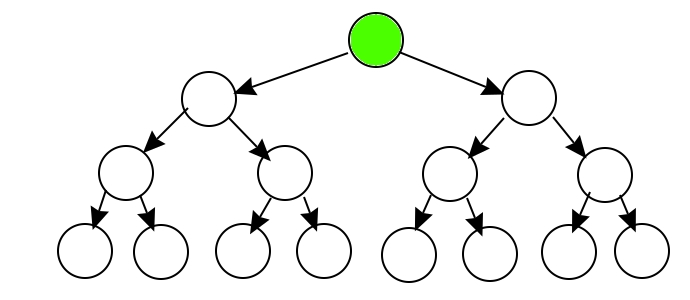
\includegraphics[width=\linewidth]{search_tree_example.jpg}
		}
		\only<2>{
			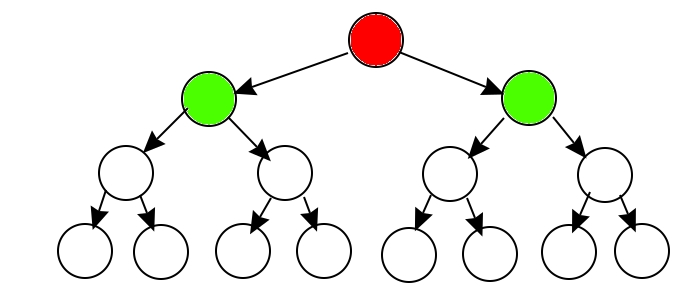
\includegraphics[width=\linewidth]{search_tree_bfs_1.jpg}
		}
		\only<3>{
			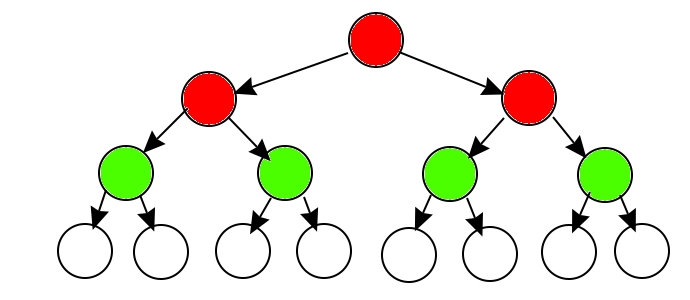
\includegraphics[width=\linewidth]{search_tree_bfs_2.jpg}
		}
		\only<4>{
			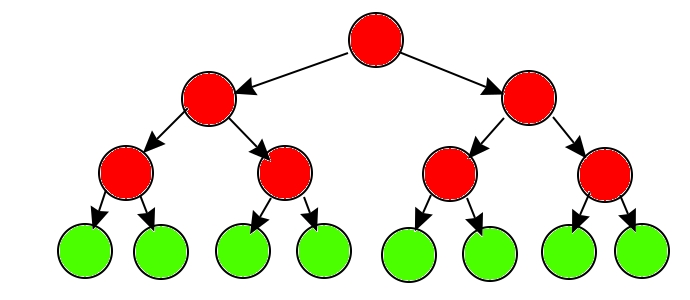
\includegraphics[width=\linewidth]{search_tree_bfs_3.jpg}
		}
	\end{figure}
\end{frame}

\begin{frame}{Breadth First Search (BFS)}
	\begin{itemize}
		\item The good:
			\pause
			\begin{itemize}
				\item Always finds the solution
				\item Optimal route to the solution
			\end{itemize}
		\pause
		\item The bad:
			\pause
			\begin{itemize}
				\item Kinda dumb...
			\end{itemize}
		\pause
		\item The ugly:
			\pause
			\begin{itemize}
				\item Memory consumption on larger graphs	
			\end{itemize}
	\end{itemize}				
\end{frame}

\subsection{Depth first search (DFS)}

\begin{frame}[fragile]{Depth First Search (DFS)}
	\begin{lstlisting}
closedNodes = {}

(*@ \textcolor{blue}{\# Last In First Out} @*)
(*@ \textcolor{blue}{openNode = Stack()} @*)

openNodes.insert(getInitialState())
while openNodes not empty 
  node = openNodes.get()
  if isGoalState(node)
    return node
  if node in closedNodes
    continue				
  for childNode in getSuccessors(node)
    if childNode not in closedNodes
      openNodes.insert(childNode)
  closedNodes.insert(node)
	\end{lstlisting}
\end{frame}

\begin{frame}{Depth First Search (DFS)}
	\begin{columns}[T]
		\begin{column}{.48\textwidth}
			\begin{figure}
			\centering
				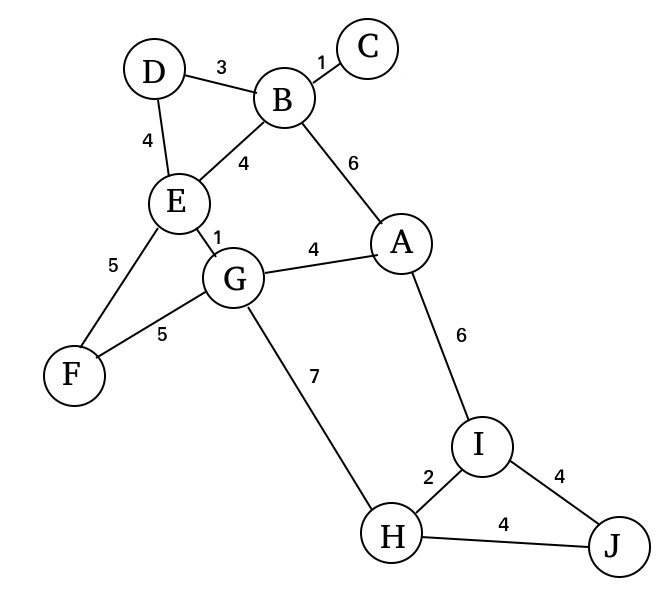
\includegraphics[width=1.3\linewidth]{example.jpg}
			\end{figure}
		\end{column}
		
		\begin{column}{.48\textwidth}
				\begin{itemize}
					\item Find a path from B to I
					\newline
					\only<1>{
						\item OPEN: {[ B ]}
						\newline
						\item CLOSED: \{\}
					}
					\only<2>{
						\item OPEN: {[ \textcolor{blue}{C, D, E, A} ]}
						\newline
						\item CLOSED: \{ \textcolor{red}{B} \}					
					}
					\only<3>{
						\item OPEN: {[ D, E, A ]}
						\newline
						\item CLOSED: \{ B, \textcolor{red}{C} \}
					}
					\only<4>{
						\item OPEN: {[ E, A ]}
						\newline
						\item CLOSED: \{ B, C, \textcolor{red}{D} \}
					}
					\only<5>{
						\item OPEN: {[ \textcolor{blue}{F, G}, A ]}
						\newline
						\item CLOSED: \{ B, C, D, \textcolor{red}{E} \}
					}
					\only<6>{
						\item OPEN: {[ G, A ]}
						\newline
						\item CLOSED: \{ B, C, D, E, \textcolor{red}{F} \}
					}
					\only<7>{
						\item OPEN: {[ \textcolor{blue}{H}, A ]}
						\newline
						\item CLOSED: \{ B, C, D, E, F, \textcolor{red}{G} \}
					}
					\only<8>{
						\item OPEN: {[ \textcolor{blue}{I, J}, A ]}
						\newline
						\item CLOSED: \{ B, C, D, E, F, G, \textcolor{red}{H} \}
					}
					\only<9>{
						\item Reached goal I
					}

				\end{itemize}
		\end{column}
	\end{columns}
\end{frame}

\begin{frame}{Depth First Search (DFS)}
	\begin{figure}
		\centering
		\only<1>{
			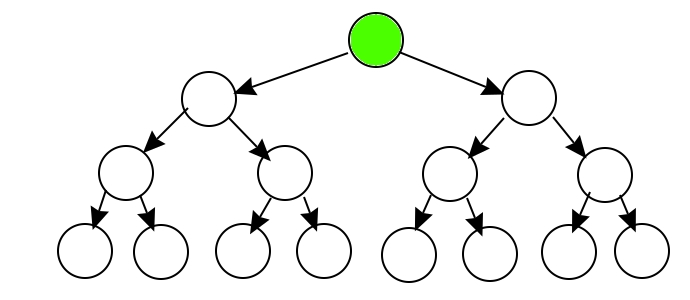
\includegraphics[width=\linewidth]{search_tree_example.jpg}
		}
		\only<2>{
			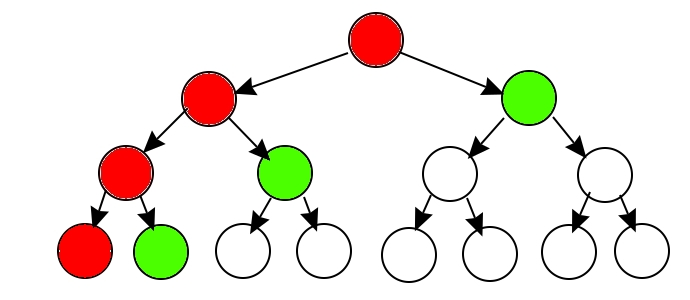
\includegraphics[width=\linewidth]{search_tree_dfs_1.jpg}
		}
		\only<3>{
			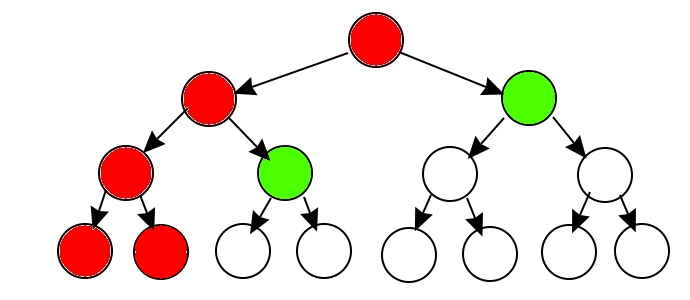
\includegraphics[width=\linewidth]{search_tree_dfs_2.jpg}
		}
		\only<4>{
			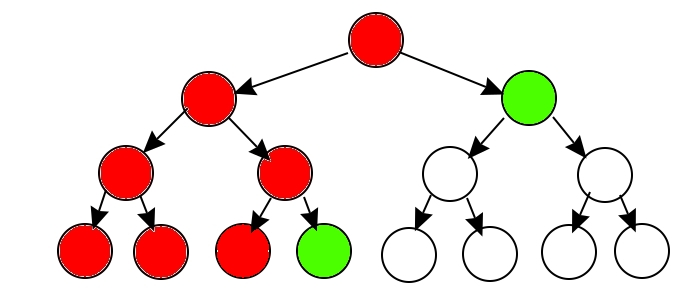
\includegraphics[width=\linewidth]{search_tree_dfs_3.jpg}
		}
		\only<5>{
			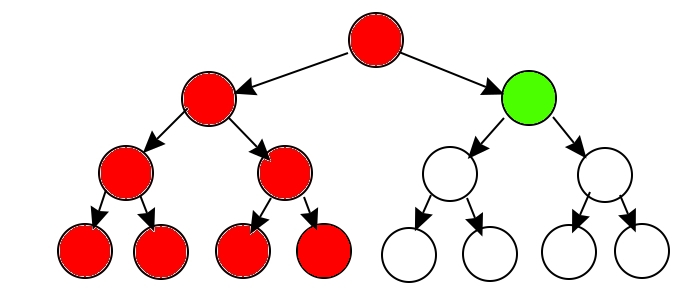
\includegraphics[width=\linewidth]{search_tree_dfs_4.jpg}
		}
		\only<6>{
			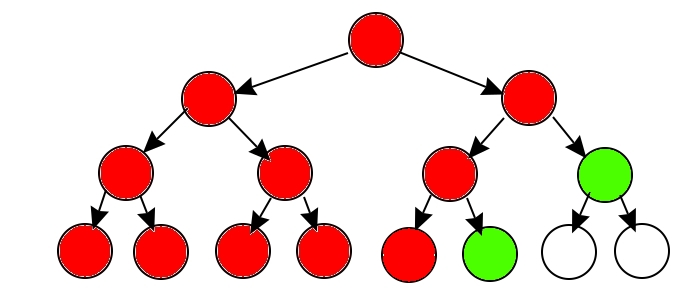
\includegraphics[width=\linewidth]{search_tree_dfs_5.jpg}
		}
	\end{figure}
\end{frame}

\begin{frame}{Depth First Search (DFS)}
	\begin{itemize}
		\item The good:
			\pause
			\begin{itemize}
				\item Always finds the solution (when taking care not to revisit states multiple times)
			\end{itemize}
		\pause
		\item The bad:
			\pause
			\begin{itemize}
				\item Not the optimal solution though
			\end{itemize}
		\pause
		\item The ugly:
			\pause
			\begin{itemize}
				\item Kinda dumb...er	
			\end{itemize}
	\end{itemize}				
\end{frame}

\subsection{Uniform cost search (UCS)}

\begin{frame}[fragile]{Uniform Cost Search (UCS)}
	\begin{lstlisting}
closedNodes = {}

(*@ \textcolor{blue}{\# Elements sorted by priority} @*)
(*@ \textcolor{blue}{openNode = PriorityQueue()} @*)

(*@ \textcolor{blue}{openNodes.insert((0, getInitialState()))} @*)
while openNodes not empty 
  (*@ \textcolor{blue}{cost, node = openNodes.get()} @*)
  if isGoalState(node)
    return node
  if node in closedNodes
    continue				
  (*@ \textcolor{blue}{for childNode, actionCost in getSuccessors(node)} @*)
    if childNode not in closedNodes
      (*@ \textcolor{blue}{openNodes.insert((cost + actionCost, childNode))} @*)
  closedNodes.insert(node)
	\end{lstlisting}
\end{frame}

\begin{frame}{Uniform Cost Search (UCS)}
	\begin{columns}[T]
		\begin{column}{.48\textwidth}
			\begin{figure}
			\centering
				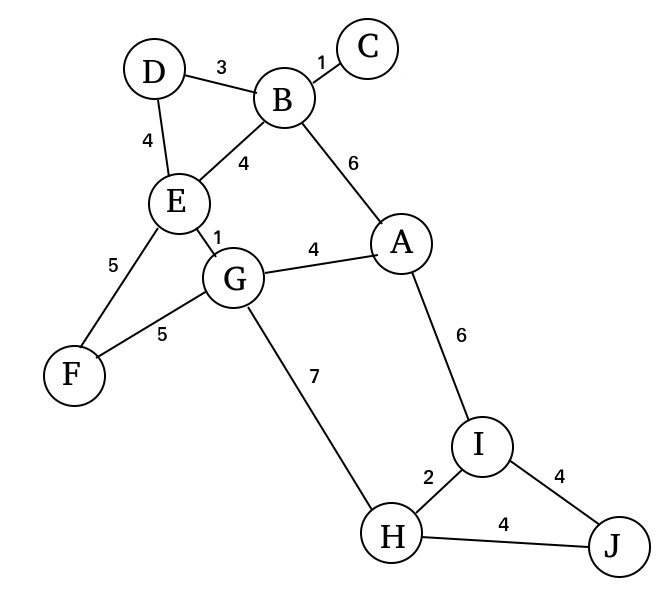
\includegraphics[width=1.3\linewidth]{example_weights.jpg}
			\end{figure}
		\end{column}
		
		\begin{column}{.48\textwidth}
				\begin{itemize}
					\item Find a path from B to I
					\newline
					\only<1>{
						\item OPEN: {[ (0, B) ]}
						\newline
						\item CLOSED: \{\}
					}
					\only<2>{
						\item OPEN: {[ \textcolor{blue}{(1, C), (3, D), (4, E), (6, A)} ]}
						\newline
						\item CLOSED: \{ \textcolor{red}{B} \}					
					}
					\only<3>{
						\item OPEN: {[ (3, D), (4, E), (6, A) ]}
						\newline
						\item CLOSED: \{ B, \textcolor{red}{C} \}
					}
					\only<4>{
						\item OPEN: {[ (4, E), (6, A) ]}
						\newline
						\item CLOSED: \{ B, C, \textcolor{red}{D} \}
					}
					\only<5>{
						\item OPEN: {[ \textcolor{blue}{(5, G)}, (6, A), \textcolor{blue}{(9, F)} ]}
						\newline
						\item CLOSED: \{ B, C, D, \textcolor{red}{E} \}
					}
					\only<6>{
						\item OPEN: {[ (6, A), (9, F), \textcolor{blue}{(12, H)} ]}
						\newline
						\item CLOSED: \{ B, C, D, E, \textcolor{red}{G} \}
					}
					\only<7>{
						\item OPEN: {[ (9, F), \textcolor{blue}{(11, I)}, (12, H) ]}
						\newline
						\item CLOSED: \{ B, C, D, E, G, \textcolor{red}{A} \}
					}
					\only<8>{
						\item OPEN: {[ (11, I), (12, H) ]}
						\newline
						\item CLOSED: \{ B, C, D, E, G, A, \textcolor{red}{F} \}
					}
					\only<9>{
						\item Reached goal I
					}

				\end{itemize}
		\end{column}
	\end{columns}
\end{frame}

\begin{frame}{Uniform Cost Search (UCS)}
	\begin{itemize}
		\item Same as BFS but with variable cost transitions
	\end{itemize}				
\end{frame}

\section{Heuristic algorithms}

\begin{frame}{Heuristic algorithms}

	\begin{itemize}
		\item You can give them some hints
		\pause
		\item They may or may not listen to you though...
	\end{itemize}

\end{frame}

\subsection{Heuristics}

\begin{frame}{What is a heuristic?}
	\begin{figure}
	\centering
		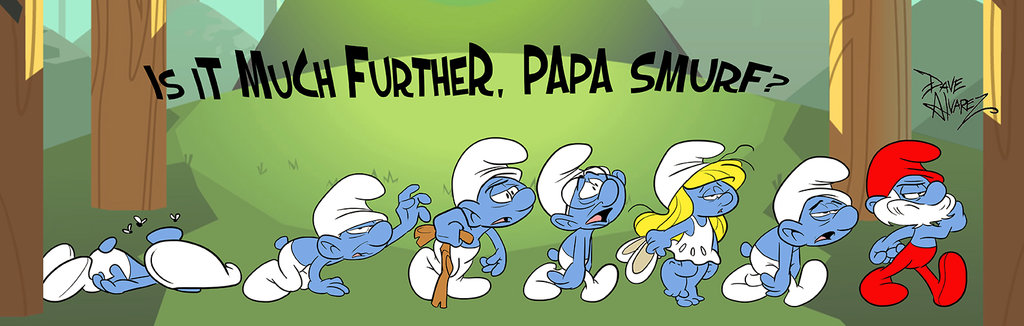
\includegraphics[width=\linewidth]{are_we_there_yet.jpg}
	\end{figure}

	\begin{itemize}
		\item Estimation of the distance to the goal
		\item Examples:
		\begin{itemize}
			\pause
			\item Manhattan distance on a grid
			\pause
			\item Euclidean distance (air distance) between cities
			\pause
			\item In our example let's use minimal number of jumps needed to get to the goal
		\end{itemize}
	\end{itemize}
\end{frame}

\begin{frame}{What is a heuristic?}
	\begin{figure}
	\centering
		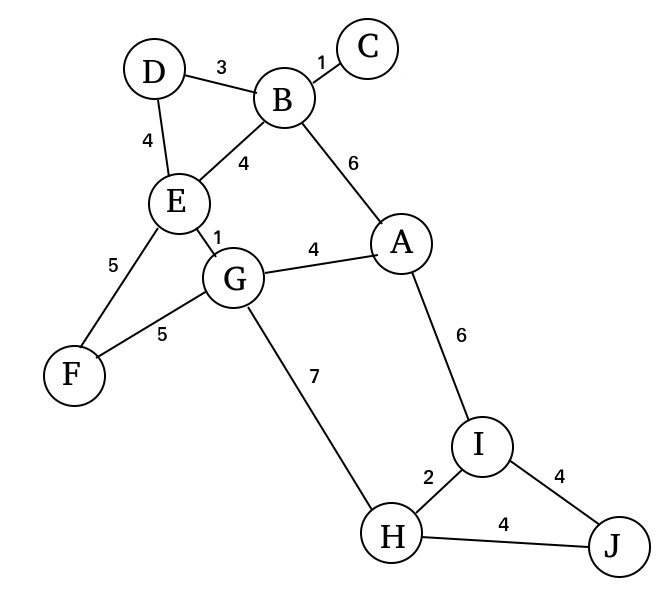
\includegraphics[width=0.7\linewidth]{example_weights.jpg}
	\end{figure}
\end{frame}

\subsection{Greedy search}

\begin{frame}[fragile]{Greedy Search}
	\begin{lstlisting}
closedNodes = {}

# Elements sorted by priority
openNode = PriorityQueue()

openNodes.insert((0, getInitialState()))
while openNodes not empty 
  cost, node = openNodes.get()
  if isGoalState(node)
    return node
  if node in closedNodes
    continue				
  for childNode, actionCost in getSuccessors(node)
    if childNode not in closedNodes
      (*@ \textcolor{blue}{openNodes.insert((h(childNode), childNode))} @*)
  closedNodes.insert(node)
	\end{lstlisting}
\end{frame}

\begin{frame}{Greedy Search}
	\begin{columns}[T]
		\begin{column}{.48\textwidth}
			\begin{figure}
			\centering
				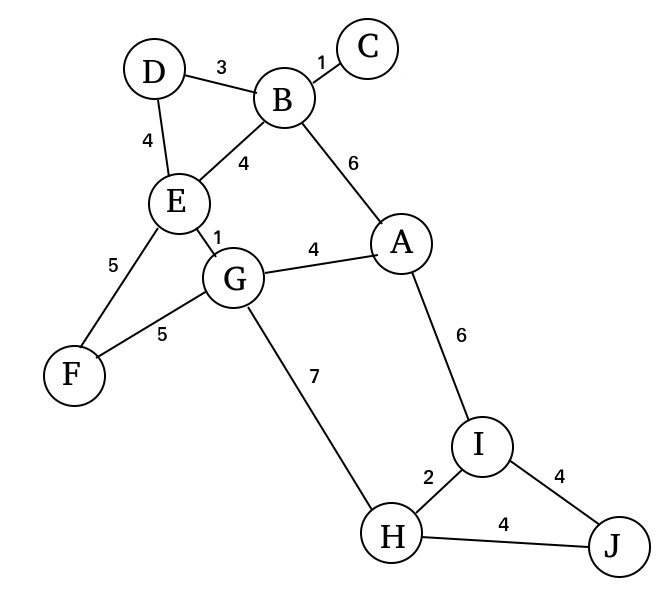
\includegraphics[width=1.3\linewidth]{example_weights.jpg}
			\end{figure}
		\end{column}
		
		\begin{column}{.48\textwidth}
				\begin{itemize}
					\item Find a path from B to I
					\newline
					\only<1>{
						\item OPEN: {[ (0, B) ]}
						\newline
						\item CLOSED: \{\}
					}
					\only<2>{
						\item OPEN: {[ \textcolor{blue}{(1, A), (3, D), (3, E), (3, C)} ]}
						\newline
						\item CLOSED: \{ \textcolor{red}{B} \}					
					}
					\only<3>{
						\item OPEN: {[ \textcolor{blue}{(0, I), (2, G)}, (3, D), (3, E), (3, C) ]}
						\newline
						\item CLOSED: \{ B, \textcolor{red}{A} \}
					}
					\only<4>{
						\item Reached goal I
					}
				\end{itemize}
		\end{column}
	\end{columns}
\end{frame}

\begin{frame}{Greedy Search}
	\begin{itemize}
		\item The good:
			\pause
			\begin{itemize}
				\item Always finds the solution (when taking care not to revisit states multiple times)
				\item Quickly finds a solution
			\end{itemize}
		\pause
		\item The bad:
			\pause
			\begin{itemize}
				\item Not the optimal solution though
			\end{itemize}
		\pause
		\item The ugly:
			\pause
			\begin{itemize}
				\item Trusts you a bit too much...
			\end{itemize}
	\end{itemize}				
\end{frame}

\subsection{A* search}

\begin{frame}[fragile]{A* Search}
	\begin{lstlisting}
closedNodes = {}

# Elements sorted by priority
openNode = PriorityQueue()

openNodes.insert((0, 0, getInitialState()))
while openNodes not empty 
  _, cost, node = openNodes.get()
  if isGoalState(node)
    return node
  if node in closedNodes
    continue			
  for childNode, actionCost in getSuccessors(node)
    if childNode not in closedNodes
      (*@ \textcolor{blue}{totalCost = actionCost + cost} @*)
      (*@ \textcolor{blue}{openNodes.insert((totalCost + h(childNode), totalCost, childNode))} @*)
  closedNodes.insert(node)
	\end{lstlisting}
\end{frame}

\begin{frame}{A* Search}
	\begin{columns}[T]
		\begin{column}{.48\textwidth}
			\begin{figure}
			\centering
				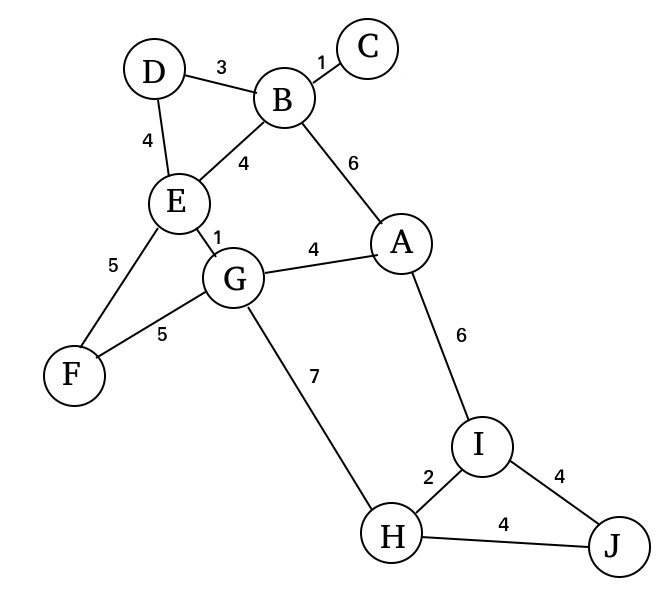
\includegraphics[width=1.3\linewidth]{example_weights.jpg}
			\end{figure}
		\end{column}
		
		\begin{column}{.48\textwidth}
				\begin{itemize}
					\item Find a path from B to I
					\newline
					\only<1>{
						\item OPEN: {[ (0, 0, B) ]}
						\newline
						\item CLOSED: \{\}
					}
					\only<2>{
						\item OPEN: {[ \textcolor{blue}{(4, 1, C), (6, 3, D), (7, 4, E), (7, 6, A)} ]}
						\newline
						\item CLOSED: \{ \textcolor{red}{B} \}					
					}
					\only<3>{
						\item OPEN: {[ (6, 3, D), (7, 4, E), (7, 6, A) ]}
						\newline
						\item CLOSED: \{ B, \textcolor{red}{C} \}
					}
					\only<4>{
						\item OPEN: {[ (7, 4, E), (7, 6, A) ]}
						\newline
						\item CLOSED: \{ B, C, \textcolor{red}{D} \}
					}
					\only<5>{
						\item OPEN: {[ \textcolor{blue}{(7, 5, G)}, (7, 6, A), \textcolor{blue}{(12, 9, F)} ]}
						\newline
						\item CLOSED: \{ B, C, D, \textcolor{red}{E} \}
					}
					\only<6>{
						\item OPEN: {[ (7, 6, A), (12, 9, F), \textcolor{blue}{(13, 12, H)} ]}
						\newline
						\item CLOSED: \{ B, C, D, E, \textcolor{red}{G} \}
					}
					\only<7>{
						\item OPEN: {[ \textcolor{blue}{(11, 11, I)}, (12, 9, F), (13, 12, H) ]}
						\newline
						\item CLOSED: \{ B, C, D, E, G, \textcolor{red}{A} \}
					}
					\only<8>{
						\item Reached goal I
					}
				\end{itemize}
		\end{column}
	\end{columns}
\end{frame}

\begin{frame}{Greedy Search}
	\begin{itemize}
		\item Always finds the solution
		\item If the given heuristic is \textbf{optimistic} the solution is optimal
	\end{itemize}			
\end{frame}

\begin{frame}
	\centering
	Live demonstration
\end{frame}

\section{Other algorithms}

\begin{frame}{Is there anything better?}
	\pause
	Well...depends...
	\pause
	\begin{itemize}
		\item Dijkstra's algorithm (same as UCS but without an exact "goal") - mostly used in networking
		\pause
		\item D* search and variations - mostly used in robotics
		\pause
		\item A* search and variations - most often the best solution for a video game pathfinding
	\end{itemize}
\end{frame}

\section{Pathfinding in video games}

\begin{frame}{Pathfinding in video games}

	\only<1>{
		\begin{columns}[T]
			\begin{column}{.26\textwidth}
				\begin{center}
					Alright there's an obvious grid...				
				\end{center}
			\end{column}
			
			\begin{column}{.70\textwidth}
				\begin{figure}
				\centering
					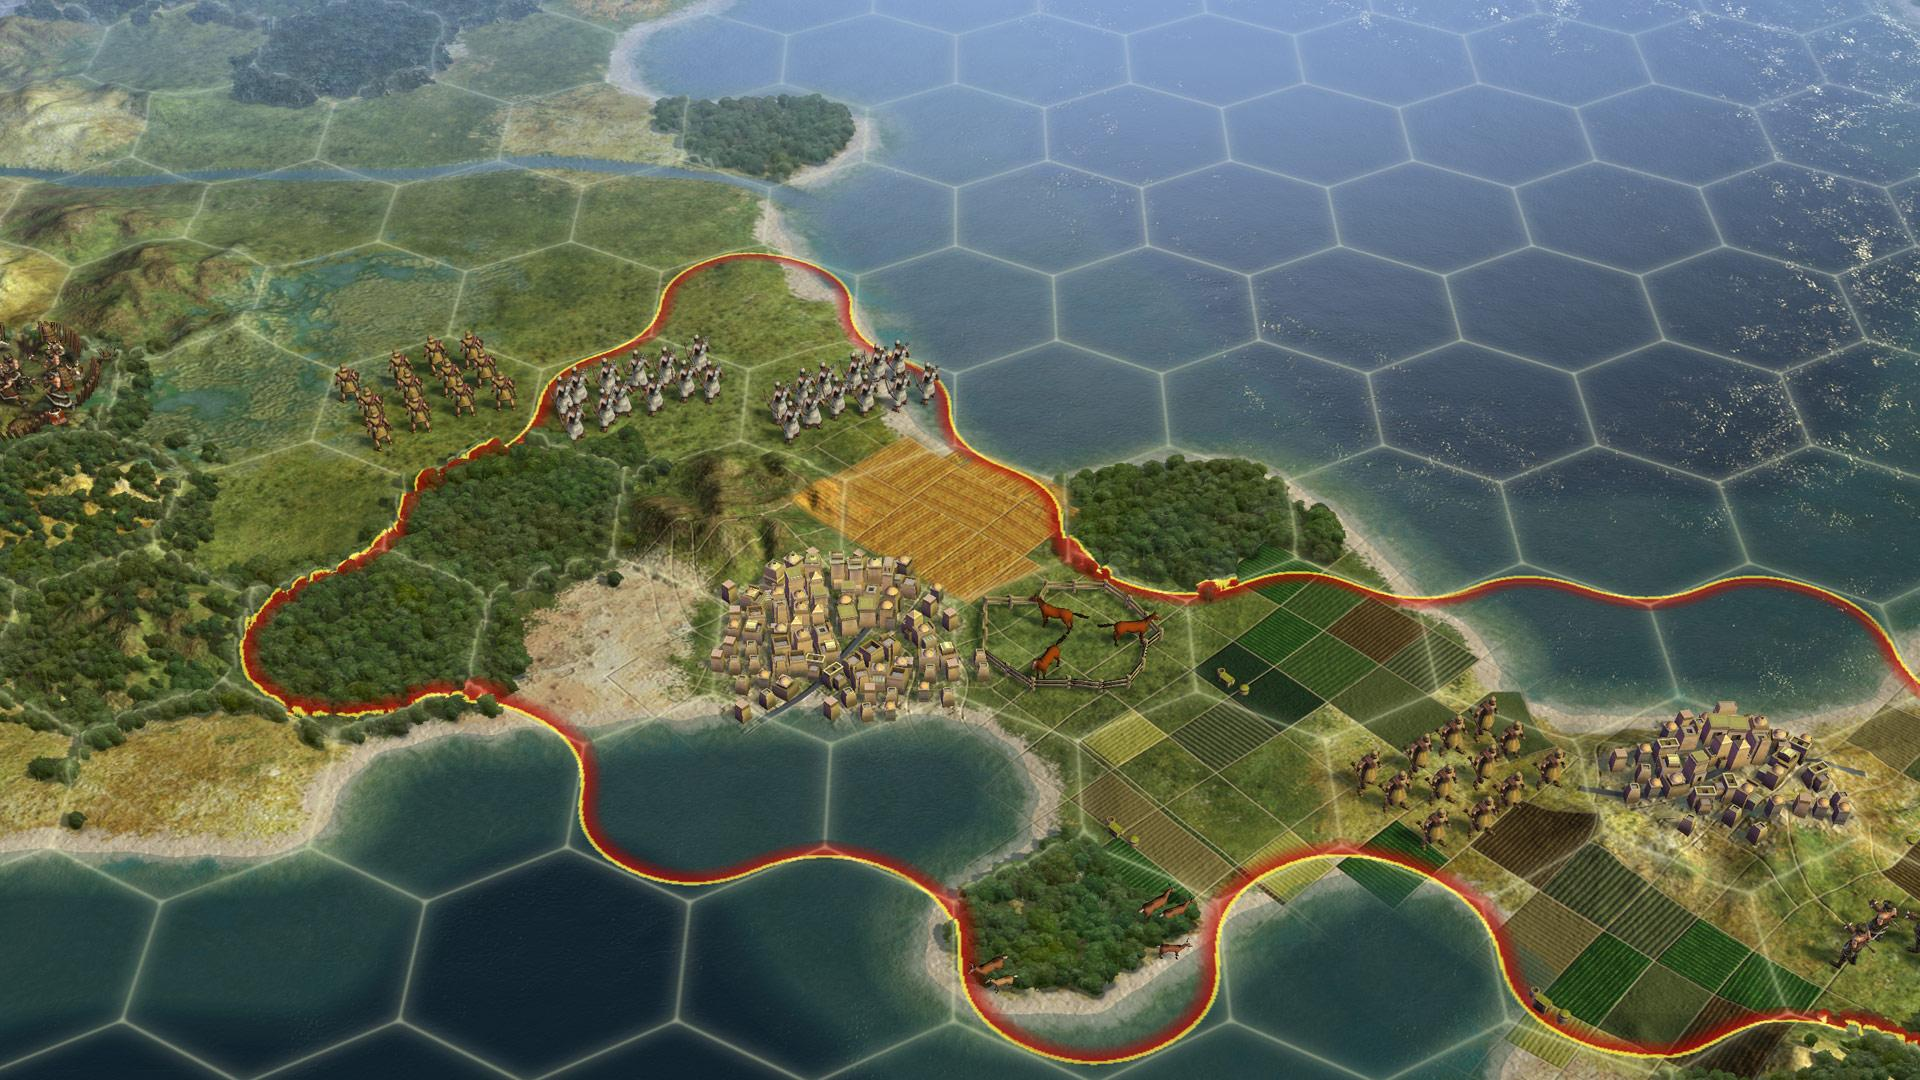
\includegraphics[width=0.8\linewidth]{civilization_grid.jpg}
				\end{figure}
				
				\begin{figure}
				\centering
					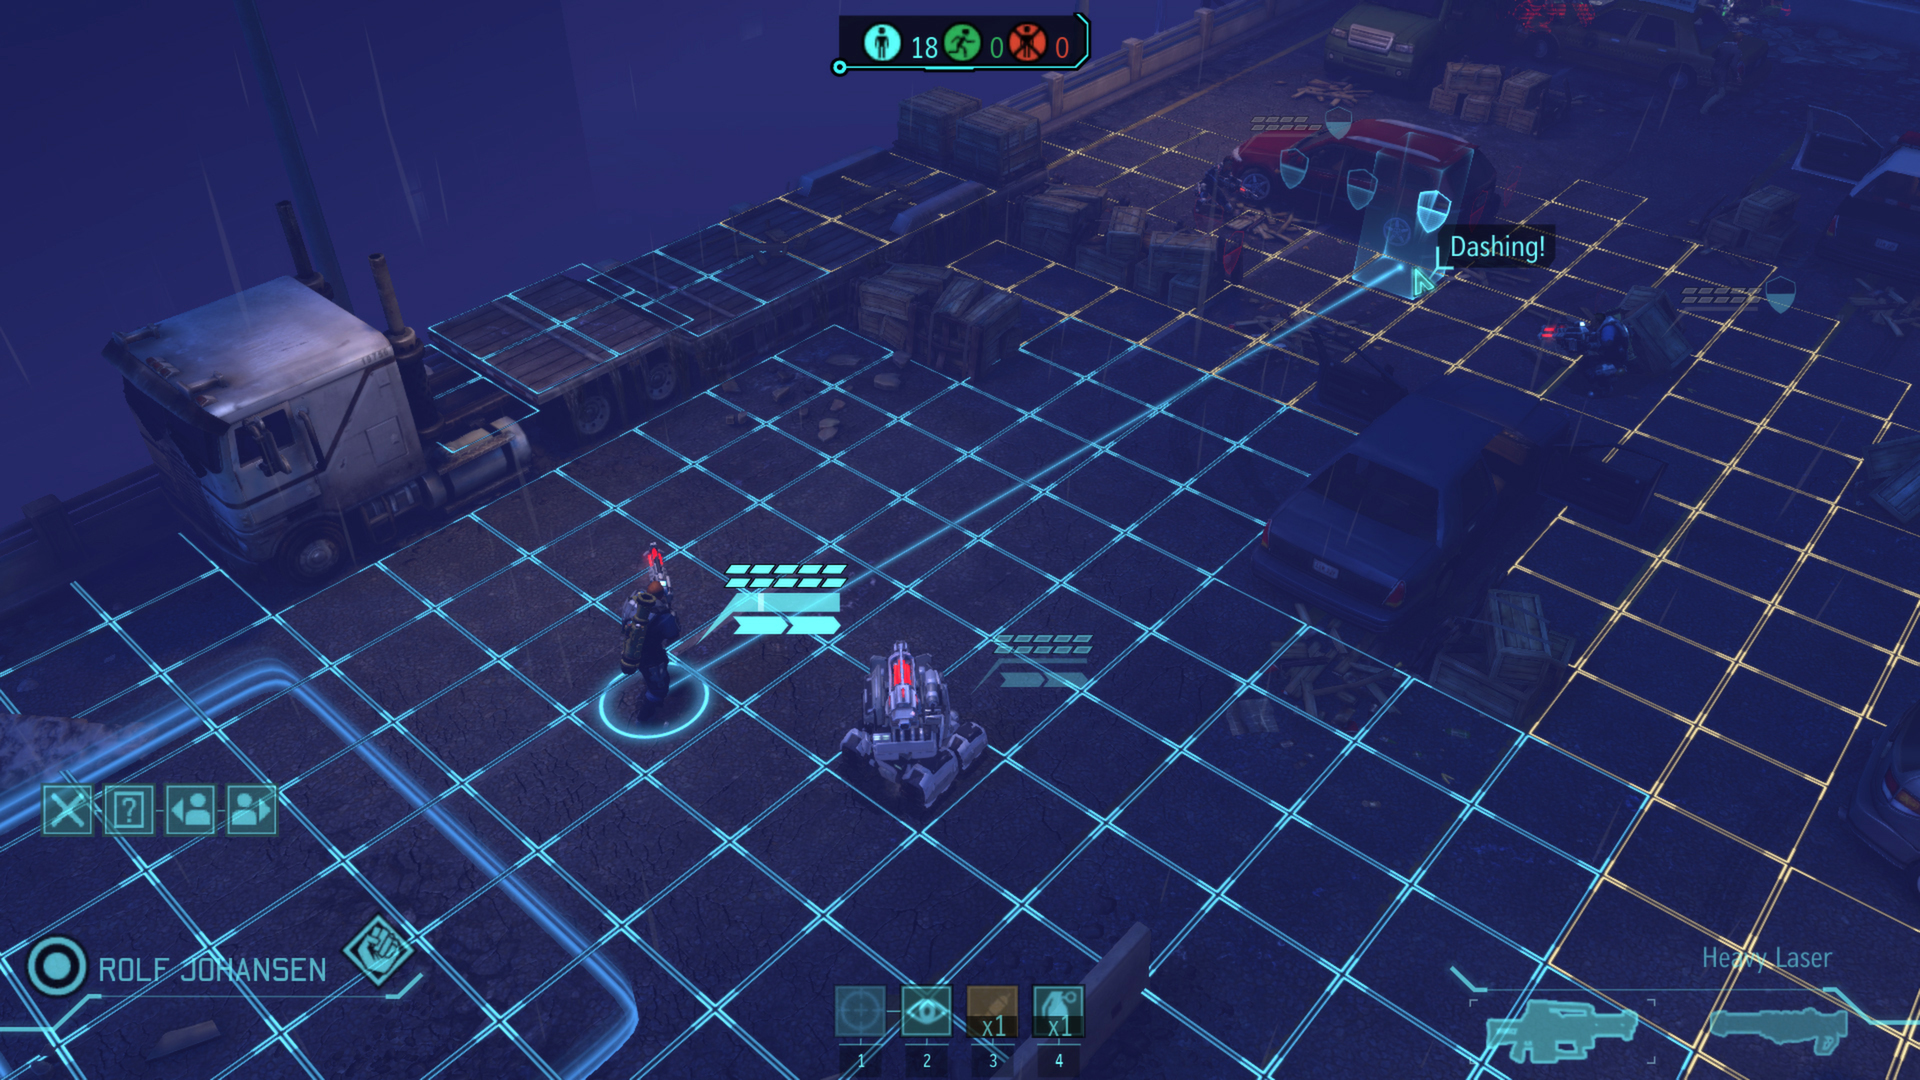
\includegraphics[width=0.8\linewidth]{xcom_grid.jpg}
				\end{figure}
			\end{column}
		\end{columns}
	}
	
	\only<2>{
		\begin{columns}[T]
			\begin{column}{.26\textwidth}
				\begin{center}
					...now what?			
				\end{center}
			\end{column}
			
			\begin{column}{.70\textwidth}
				\begin{figure}
				\centering
					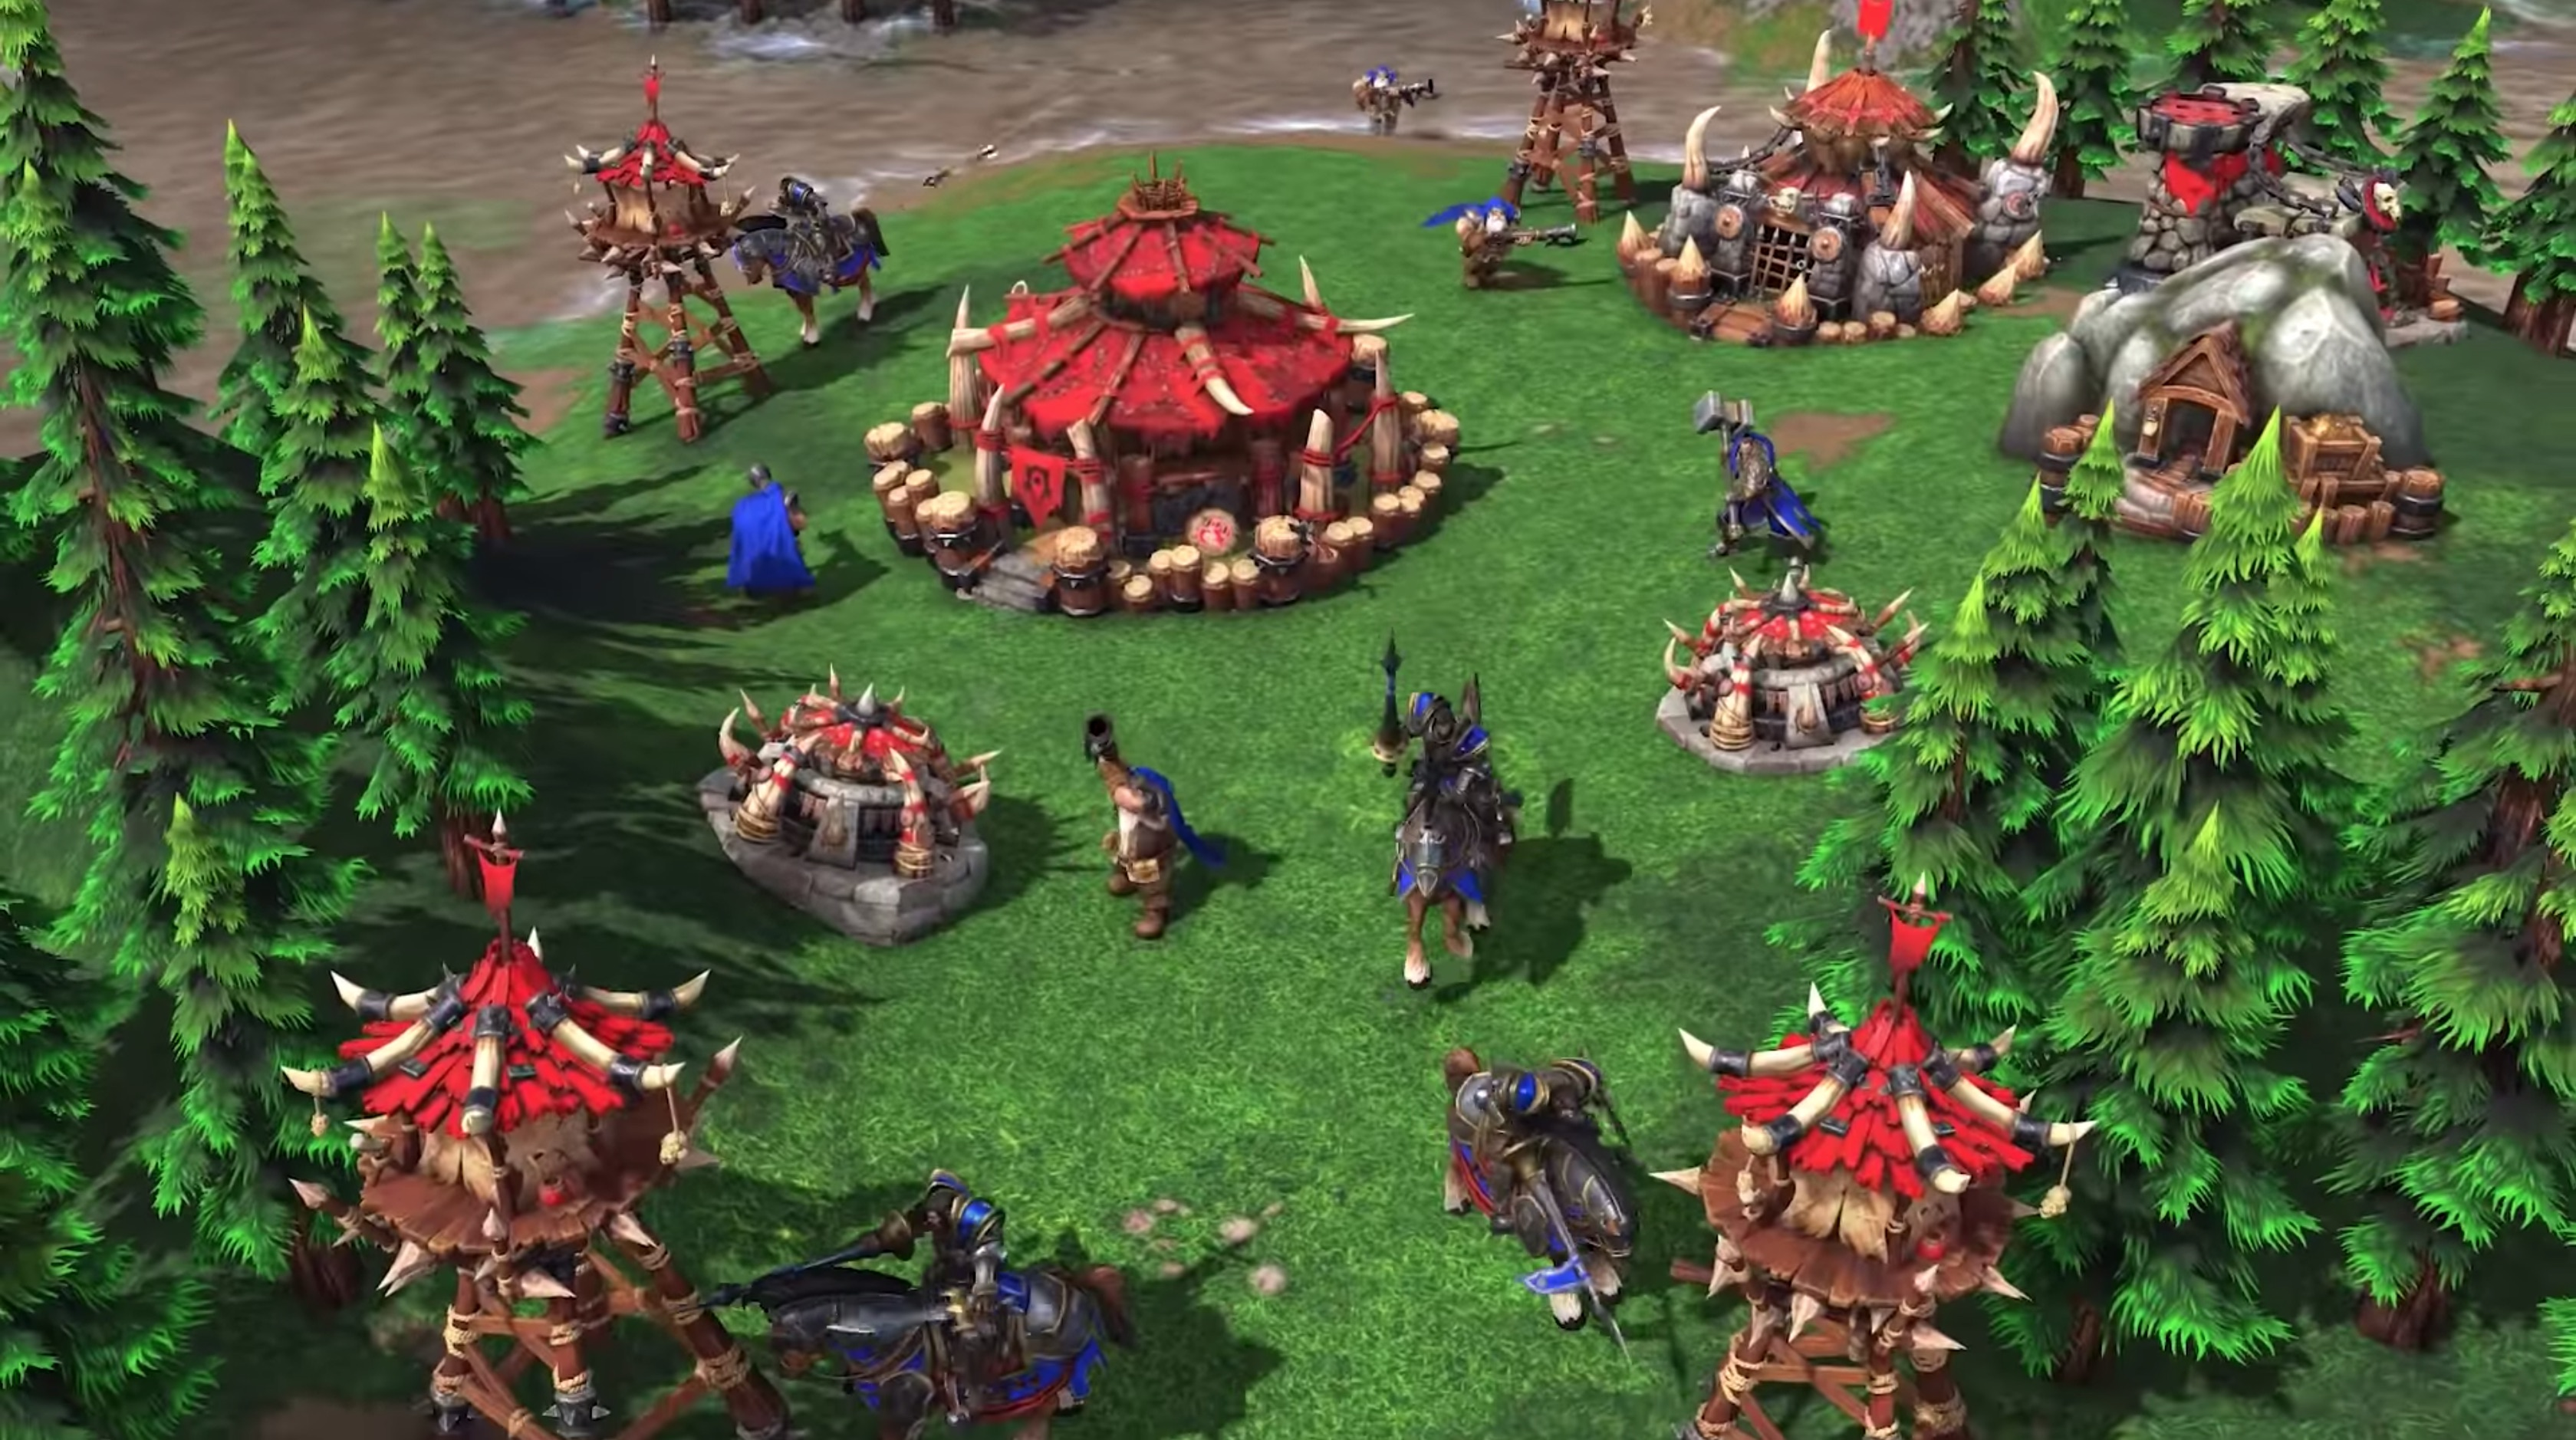
\includegraphics[width=\linewidth]{warcraft_grid.jpg}
				\end{figure}
			\end{column}
		\end{columns}
	}
\end{frame}

\begin{frame}{Visibility graph}
	\begin{figure}
	\centering
		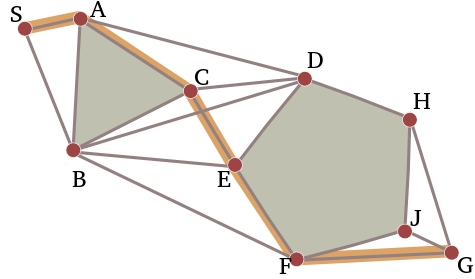
\includegraphics[width=\linewidth]{visibility_graph.jpg}
	\end{figure}
\end{frame}

\begin{frame}{Divide and conquer}
	\begin{itemize}
		\item Divide the whole grid into several smaller pieces
		\item Agents don't need to find a path on the whole grid at once
		\item Easier to modify the graph in case of frequent smaller changes in the terrain
	\end{itemize}
\end{frame}

\begin{frame}
	\centering
	Any questions?
	
	{\tiny Plz no difficult ones}
\end{frame}

\end{document}